\documentclass[border=1pt]{standalone}
\usepackage[scaled=0.92]{helvet}
\renewcommand{\familydefault}{\sfdefault}
\usepackage{amsmath}
\usepackage{tikz}
\usetikzlibrary{arrows.meta,fit,calc,backgrounds}
% colours shared with Fig. 4: blue = trained, teal = stored code y_{t-1}, red = extra robot cost
\definecolor{ours}{HTML}{DCEAFB}\definecolor{oursline}{HTML}{2A78D6}\definecolor{ourstxt}{HTML}{0D366B}
\definecolor{ref}{HTML}{D7F0EC}\definecolor{refline}{HTML}{23998A}\definecolor{reftxt}{HTML}{14655B}
\definecolor{fixed}{HTML}{FFF3C4}\definecolor{fixedline}{HTML}{C9A227}\definecolor{fixedtxt}{HTML}{4F3D05}
\definecolor{cost}{HTML}{FBE3E1}\definecolor{costline}{HTML}{C8463D}\definecolor{costtxt}{HTML}{7A1F19}
\definecolor{panel}{HTML}{EDEDED}\definecolor{txt}{HTML}{333333}
\begin{document}
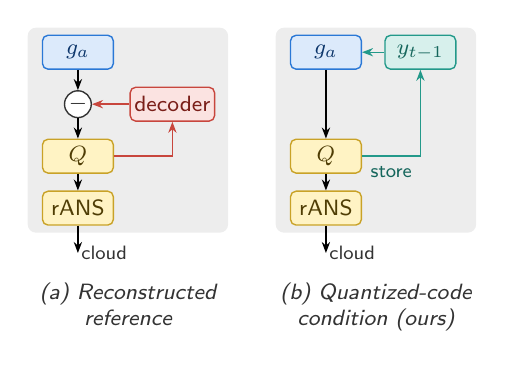
\begin{tikzpicture}[
  font=\footnotesize, text=txt,
  >={Stealth[length=1.4mm]}, line width=0.5pt,
  box/.style={rounded corners=2pt, minimum height=4.3mm, minimum width=9mm, inner sep=1.5pt, align=center},
  ga/.style={box, fill=ours, draw=oursline, text=ourstxt},
  opstep/.style={box, fill=fixed, draw=fixedline, text=fixedtxt},
  refb/.style={box, fill=ref, draw=refline, text=reftxt},
  costb/.style={box, fill=cost, draw=costline, text=costtxt},
  op/.style={circle, draw=txt, fill=white, inner sep=0pt, minimum size=3.4mm},
  pan/.style={fill=panel, rounded corners=3pt, inner sep=2.5pt},
  subcap/.style={font=\footnotesize\itshape, anchor=north, align=center},
]
% shared row positions (cm), top to bottom
\def\rA{0}\def\rB{-0.66}\def\rC{-1.32}\def\rD{-1.98}\def\rE{-2.55}
\def\side{1.2}

% ---------- (a) reconstructed reference ----------
\begin{scope}[xshift=0cm]
\node[ga] (a1) at (0,\rA) {$g_a$};
\node[op]  (a2) at (0,\rB) {$-$};
\node[opstep]  (a3) at (0,\rC) {$Q$};
\node[opstep]  (a4) at (0,\rD) {rANS};
\node[costb] (a5) at (\side,\rB) {decoder};
\coordinate (a6) at (0,\rE);
\draw[->] (a1)--(a2); \draw[->] (a2)--(a3); \draw[->] (a3)--(a4);
\draw[->] (a4)--(a6) node[right, font=\scriptsize, inner sep=1pt]{cloud};
\draw[->, costline] (a3.east) -| (a5.south);
\draw[->, costline] (a5)--(a2);
\coordinate (aL) at (-0.55,\rA); \coordinate (aR) at (\side+0.62,\rA);
\begin{scope}[on background layer]
\node[pan, fit=(a1)(a4)(a5)(aL)(aR)] (pa) {};
\end{scope}
\end{scope}

% ---------- (b) quantized-code condition (ours) ----------
% rows match (a): Q and rANS sit on the same rows as in (a)
\begin{scope}[xshift=3.15cm]
\node[ga] (b1) at (0,\rA) {$g_a$};
\node[opstep]  (b2) at (0,\rC) {$Q$};
\node[opstep]  (b4) at (0,\rD) {rANS};
\node[refb]  (b5) at (\side,\rA) {$y_{t-1}$};
\coordinate (b6) at (0,\rE);
\draw[->] (b1)--(b2); \draw[->] (b2)--(b4);
\draw[->] (b4)--(b6) node[right, font=\scriptsize, inner sep=1pt]{cloud};
\draw[->, refline] (b2.east) -| node[pos=0.25, below, font=\scriptsize, text=reftxt]{store} (b5.south);
\draw[->, refline] (b5)--(b1);
\coordinate (bL) at (-0.55,\rA); \coordinate (bR) at (\side+0.62,\rA);
\begin{scope}[on background layer]
\node[pan, fit=(b1)(b4)(b5)(bL)(bR)] (pnb) {};
\end{scope}
\end{scope}

% sub-captions aligned on one baseline
\path (pa.south) ++(0,-0.5) coordinate (capy);
\node[subcap] at (pa.south |- capy) {(a) Reconstructed\\ reference};
\node[subcap] at (pnb.south |- capy) {(b) Quantized-code\\ condition (ours)};

\end{tikzpicture}
\end{document}
